% Created 2017-11-16 Thu 21:40
% Intended LaTeX compiler: pdflatex
\documentclass[presentation]{beamer}
\usepackage[utf8]{inputenc}
\usepackage[T1]{fontenc}
\usepackage{graphicx}
\usepackage{grffile}
\usepackage{longtable}
\usepackage{wrapfig}
\usepackage{rotating}
\usepackage[normalem]{ulem}
\usepackage{amsmath}
\usepackage{textcomp}
\usepackage{amssymb}
\usepackage{capt-of}
\usepackage{hyperref}
\usepackage{minted}
\usepackage{helvet}
\usepackage{xcolor}
\definecolor{lgray}{rgb}{0.90,0.90,0.90}
\usetheme{Boadilla}
\usecolortheme{seahorse}
\author{Dale J. Barr}
\date{University of Glasgow}
\title{Research Cycle 08: General Linear Model}
\hypersetup{
 pdfauthor={Dale J. Barr},
 pdftitle={Research Cycle 08: General Linear Model},
 pdfkeywords={},
 pdfsubject={},
 pdfcreator={Emacs 24.5.1 (Org mode 8.3.4)}, 
 pdflang={English}}
\begin{document}

\maketitle

\section*{Slides}
\label{sec:org209b55c}

\begin{frame}[label={sec:org519e389}]{What is the ``General Linear Model'' (GLM)?}
\begin{definition}[General Linear Model or GLM]
A general mathematical framework for expressing relationships
among variables
\end{definition}

\begin{itemize}
\item Differs from the ``cookbook'' approach to statistics

\begin{itemize}
\item \(t\)-test, ANOVA, ANCOVA, \(\chi^2\) test, regression, correlation, etc.
\end{itemize}

\item Can express/test linear relationships between a numerical dependent
variable and any combination of independent variables (categorical
or continuous)

\item Can even be generalized to categorial dependent variables (through
``Generalized Linear Models''; \alert{NB}: advanced)
\end{itemize}
\end{frame}






\begin{frame}[label={sec:org5caa19b}]{ANOVA, Regression, ANCOVA}
\begin{columns}
\begin{column}[t]{.33\columnwidth}
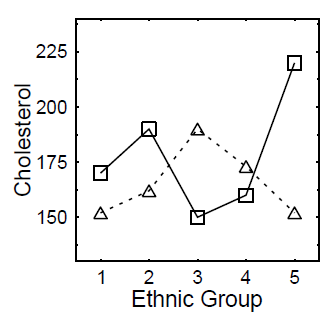
\includegraphics[width=.9\linewidth]{08_glm_img/CholesterolByEthnic.png}

\begin{center}\begin{scriptsize}
Fig 1a.  Cholesterol levels by ethnic group and gender (male=sqr, female=tri).
\end{scriptsize}\end{center}
\end{column}

\begin{column}[t]{.33\columnwidth}
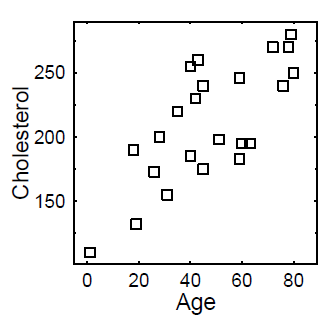
\includegraphics[width=.9\linewidth]{08_glm_img/CholesterolByAge.png}

\begin{center}\begin{scriptsize}
Fig 1a.  Cholesterol levels by age.
\end{scriptsize}\end{center}
\end{column}

\begin{column}[t]{.34\columnwidth}
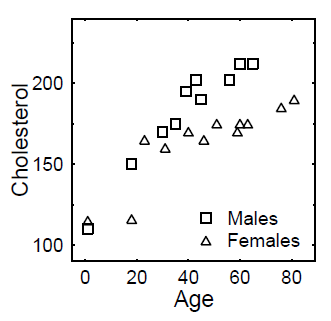
\includegraphics[width=.9\linewidth]{08_glm_img/CholesterolByGenderAge.png}

\begin{center}\begin{scriptsize}
Fig 1a.  Cholesterol levels by age and gender.
\end{scriptsize}\end{center}
\end{column}
\end{columns}
\end{frame}


\begin{frame}[label={sec:org39d43bb}]{How the GLM represents relationships}
\begin{center}
\begin{tabular}{ll}
\hline
Component of GLM & Notation\\
\hline
DV & \(Y\)\\
Grand Average & \(\mu\) ``mu''\\
Main Effects & \(A, B, C, \ldots\)\\
Interactions & \(AB, AC, BC, ABC, \ldots\)\\
Random Error & \(S(Group)\)\\
\hline
\end{tabular}
\end{center}

\begin{scriptsize}
\begin{tabular}{c@{\hspace{6pt}}@{=}@{\hspace{6pt}}c@{\hspace{6pt}}@{+}@{\hspace{6pt}}c@{\hspace{6pt}}@{+}@{\hspace{6pt}}c@{\hspace{6pt}}@{+}@{\hspace{6pt}}c}
Score & Grand Avg. & Main Effects    & Interactions          & Error\\
  $Y$ & $\mu$         & $A+B+C+ \ldots$ & $AB+AC+BC+ABC+\ldots$ & $S(Group)$ \\
\end{tabular}
\end{scriptsize}

\begin{itemize}
\item Components of the model are estimated from the observed data
\item Tests are performed ( \(F\) ) to see whether its variability is too large to be introduced by chance
\end{itemize}
\end{frame}


\begin{frame}[label={sec:org7b16a49}]{An example: Simple Linear Regression}
\begin{columns}
\begin{column}{.4\columnwidth}
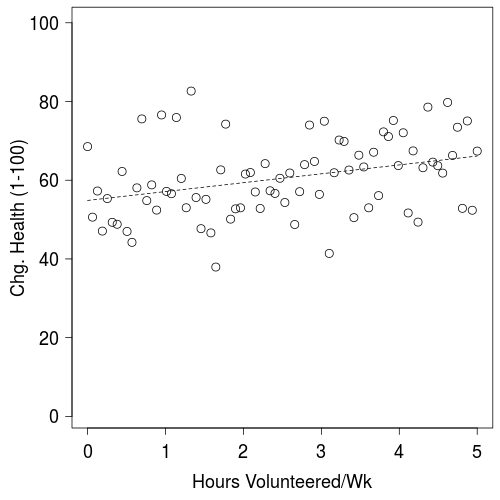
\includegraphics[width=.9\linewidth]{08_glm_img/satisfaction.png}
\end{column}
\end{columns}

\begin{center}
\begin{tabular}{c@{\hspace{6pt}}@{=}@{\hspace{6pt}}c@{\hspace{6pt}}@{+}@{\hspace{6pt}}c@{$\times$}c@{\hspace{6pt}}@{+}@{\hspace{6pt}}c}
 $Y_i$   & $\mu$    & $b$   & $X_i$   & $e_i$   \\
 Score_i & Baseline & Slope & Hours_i & Error_i \\
 $Y_i$   & $50$     & $3$   & $X_i$   & $e_i$   \\
\end{tabular}

$e_i \sim N(\mu=0, \sigma^2=10)$
\end{center}
\end{frame}

\section*{One-Factor Analysis of Variance}
\label{sec:orgc2d4fee}

\begin{frame}[label={sec:org378e3be}]{Making comparisons across groups}
\begin{example}[Spelling]
You wish to compare the benefits of three different spelling programs.  Do
these programs yield differences in spelling performance?
\end{example}

\(H_0: \mu_1 = \mu_2 = \mu_3\)

\begin{alertblock}{Factors and Levels}
Factor: a categorical variable that is used to divide subjects into
groups, usually to draw some comparison.  Factors are composed of
different \emph{levels}.  \alert{Do not confuse factors with levels!}
\end{alertblock}
\end{frame}



\begin{frame}[label={sec:org3a09c0a}]{Means, Variability, and Deviation Scores}
\begin{columns}
\begin{column}{.3\columnwidth}
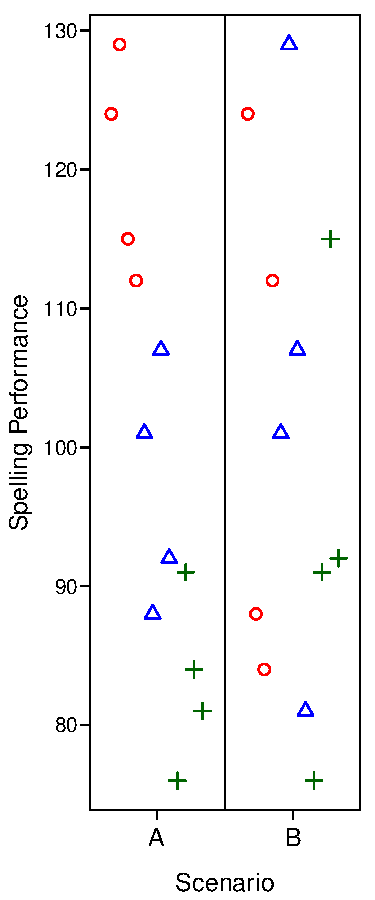
\includegraphics[width=.9\linewidth]{08_glm_img/spelling-00.pdf}
\end{column}

\begin{column}{.7\columnwidth}
\end{column}
\end{columns}
\end{frame}

\begin{frame}[label={sec:org7555801}]{Means, Variability, and Deviation Scores}
\begin{columns}
\begin{column}{.3\columnwidth}
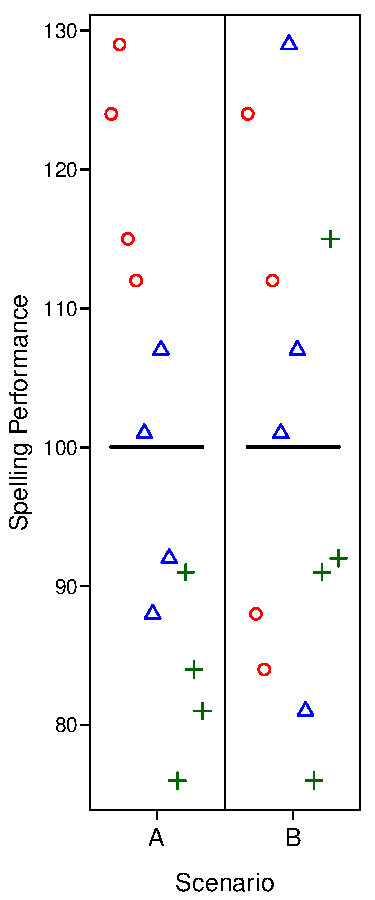
\includegraphics[width=.9\linewidth]{08_glm_img/spelling-01.pdf}
\end{column}

\begin{column}{.7\columnwidth}
\(Y_{..} = \frac{\sum_{ij} Y_{ij}}{N}\)
\end{column}
\end{columns}
\end{frame}

\begin{frame}[label={sec:orgdc8b882}]{Means, Variability, and Deviation Scores}
\begin{columns}
\begin{column}{.3\columnwidth}
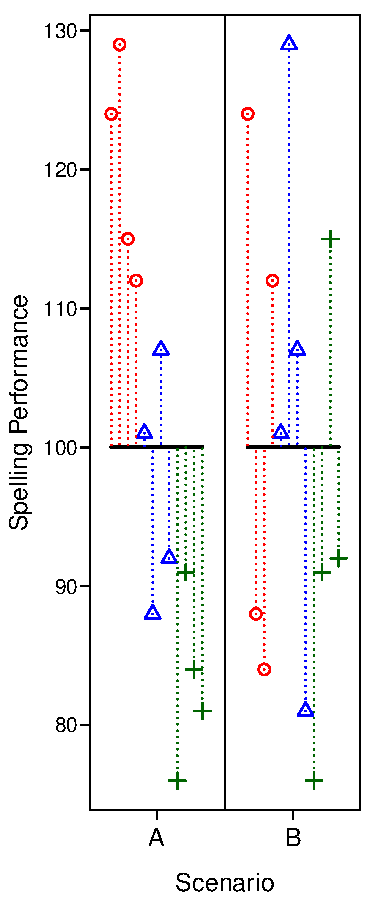
\includegraphics[width=.9\linewidth]{08_glm_img/spelling-02.pdf}
\end{column}

\begin{column}{.7\columnwidth}
grand mean $Y_{..} = \frac{\sum_{ij} Y_{ij}}{N}$\\[6pt]
$SD_Y = \sqrt{\frac{\sum_{ij} \left(Y_{ij}-Y_{..}\right)^2}{N}}$\\[6pt]
deviation score: $Y_{ij} - Y_{..}$
\end{column}
\end{columns}
\end{frame}

\begin{frame}[label={sec:orga7d2341}]{GLM for One-Factor ANOVA}
\begin{columns}
\begin{column}{.3\columnwidth}
\only<1| handout:0>{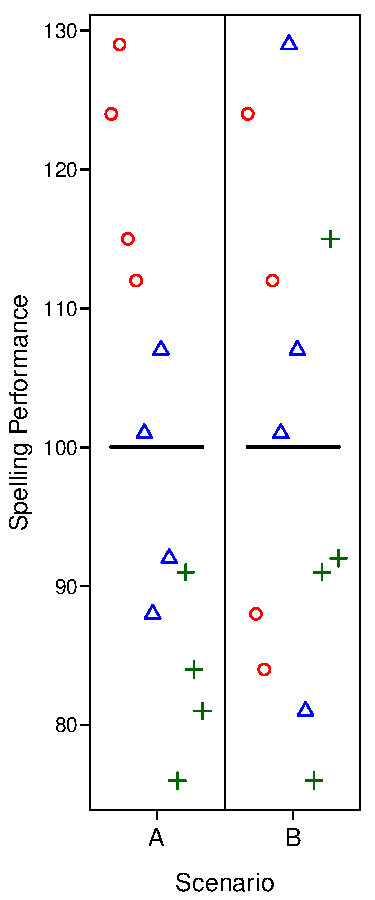
\includegraphics[scale=.5]{08_glm_img/spelling-01.pdf}}
\only<2| handout:0>{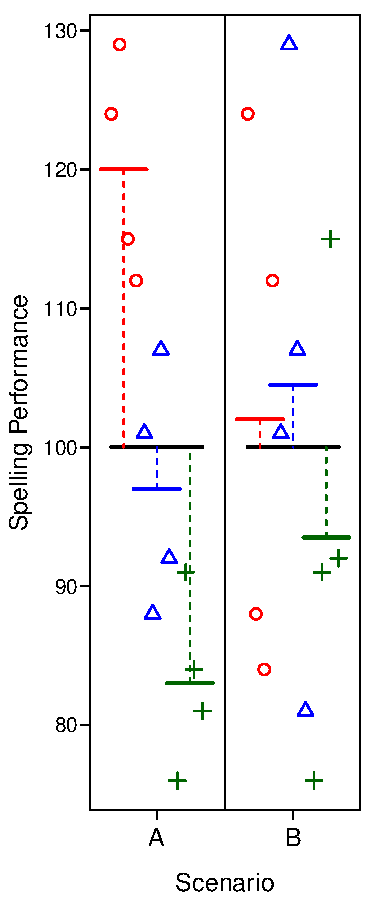
\includegraphics[scale=.5]{08_glm_img/spelling-03.pdf}}
\only<3-| handout:1>{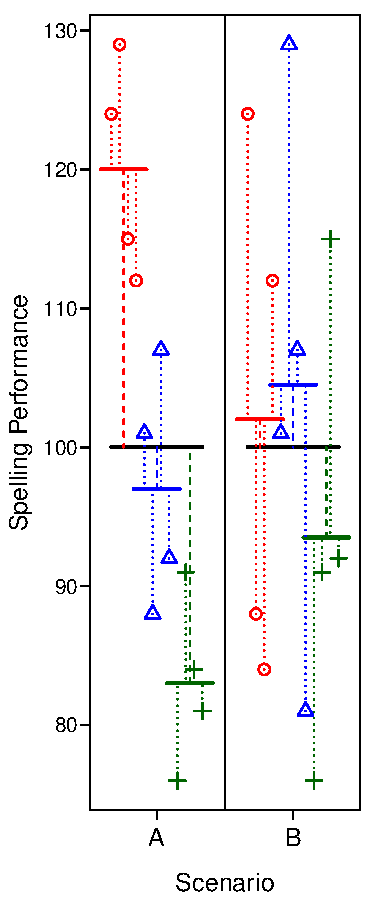
\includegraphics[scale=.5]{08_glm_img/spelling-05.pdf}}
\end{column}

\begin{column}[t]{.7\columnwidth}
\only<1| handout:0>{$Y_{ij} = \mu$\\}
\only<2| handout:0>{$Y_{ij} = \mu + A_i$\\}
\only<3-| handout:1>{$Y_{ij} = \mu + A_i + S(A)_{ij}$\\}

\begin{block}<4->{Estimation Equations}
\begin{eqnarray*}
\hat{\mu} &=& Y_{..} \\
\hat{A_i} &=& Y_{i.}-\hat{\mu}\\
\widehat{S(A)}_{ij} &=& Y_{ij} - \hat{\mu} - \hat{A_i}
\end{eqnarray*}
\end{block}

\only<4->{Note that $\sum_{i} \hat{A_i} = 0$ and $\sum_{ij} \widehat{S(A)}_{ij} = 0$}
\end{column}
\end{columns}
\end{frame}

\begin{frame}[label={sec:orgfb5bcf0}]{Sources of Variance}
\begin{columns}
\begin{column}{.3\columnwidth}
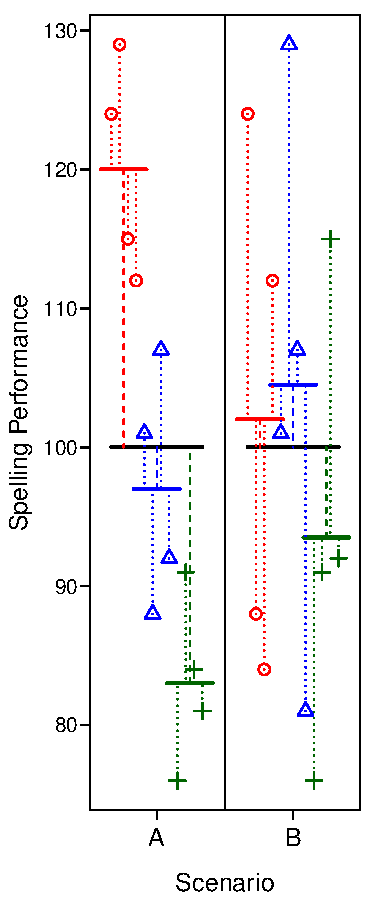
\includegraphics[scale=.5]{08_glm_img/spelling-05.pdf}
\end{column}

\begin{column}{.7\columnwidth}
\(Y_{ij} = \mu + A_i + S(A)_{ij}\)

\begin{eqnarray*}
Y_{ij}-\mu &=& A_i + S(A)_{ij}\\
individual &=& group + random
\end{eqnarray*}

\begin{block}{Sum of Squares (SS)}
A measure of variability consisting of the sum of squared \emph{deviation}
scores, where a deviation score is a score minus a mean.
\end{block}

\(SS_{A} = \sum \left(Y_{i.}-\mu\right)^2\)
\end{column}
\end{columns}
\end{frame}

\begin{frame}[label={sec:org79855a1}]{Decomposition Matrix}
\begin{columns}
\begin{column}{.25\columnwidth}
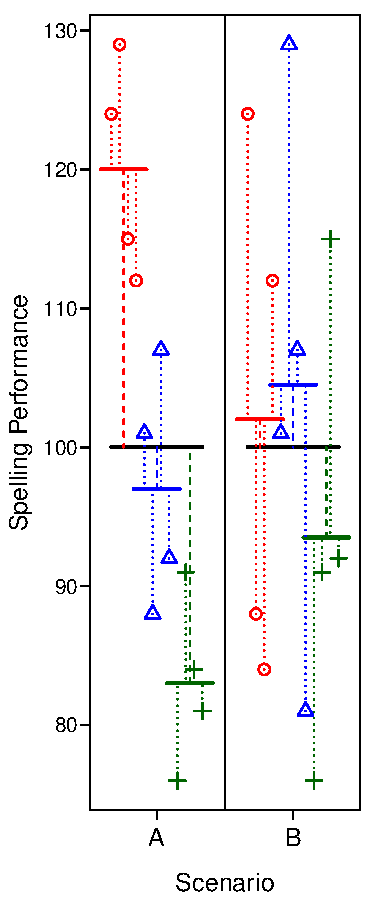
\includegraphics[scale=.5]{08_glm_img/spelling-05.pdf}
\end{column}

\begin{column}{.75\columnwidth}
\begin{center}
\begin{scriptsize}
$\hat{\mu}=100$

$\hat{A_1}=120-100=20$

$\hat{A_2}=97-100=-3$

$\hat{A_3}=83-100=-17$
\end{scriptsize}
\end{center}

\begin{center}
\begin{scriptsize}
\begin{tabular}{rr@{\hspace{6pt}}@{=}@{\hspace{6pt}}r@{\hspace{6pt}}@{+}@{\hspace{6pt}}r@{\hspace{6pt}}@{+}@{\hspace{6pt}}r}
&$Y_{ij}$ & $\hat{\mu}$ & $\hat{A_i}$ & $\widehat{S(A)}_{ij} \\ \hline
&124 & 100 &  20 &  4 \\
&129 & 100 &  20 &  9 \\
&115 & 100 &  20 & -5 \\
&112 & 100 &  20 & -8 \\
&101 & 100 &  -3 &  4 \\
& 88 & 100 &  -3 & -9 \\
&107 & 100 &  -3 & 10 \\
& 92 & 100 &  -3 & -5 \\
& 76 & 100 & -17 & -7 \\
& 91 & 100 & -17 &  8 \\
& 84 & 100 & -17 &  1 \\
& 81 & 100 & -17 & -2 \\ \hline
$SS=$ & 123318 & 120000 & 2792 & 526 \\
\end{tabular}
\end{scriptsize}
\end{center}
\end{column}
\end{columns}
\end{frame}

\begin{frame}[label={sec:org6e0477a}]{Logic of ANOVA}
\begin{columns}
\begin{column}{.25\columnwidth}
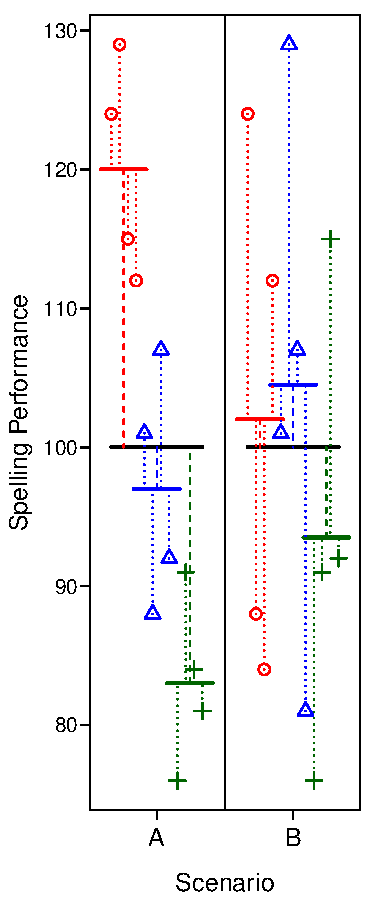
\includegraphics[scale=.5]{08_glm_img/spelling-05.pdf}
\end{column}

\begin{column}{.75\columnwidth}
\begin{itemize}
\item Compare two estimates of the variability, the \emph{between-group}
estimate (SS\_\{between\}) and the \emph{within-group} estimate (SS\_\{within\})
\item If \(H_0: \mu_1=\mu_2=\mu_3\) is true, then these two measures
estimate the same quantity.
\item The extent to which the between-group variability exceeds the
within-group variability gives evidence against \(H_0: \mu_1=\mu_2=\mu_3\).
\end{itemize}
\end{column}
\end{columns}
\end{frame}



\begin{frame}[label={sec:org8d4ad61}]{Calculating SS\_\{between\} and SS\_\{within\}}
\begin{columns}
\begin{column}{.25\columnwidth}
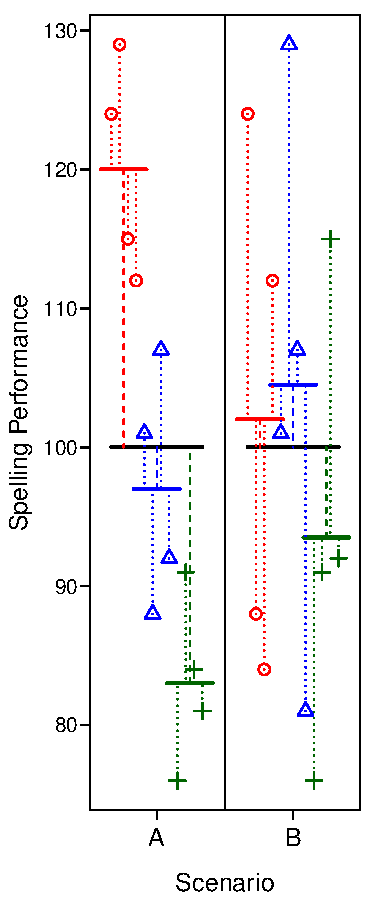
\includegraphics[scale=.5]{08_glm_img/spelling-05.pdf}
\end{column}

\begin{column}{.75\columnwidth}
\begin{center}
\begin{scriptsize}
\begin{tabular}{rr@{\hspace{6pt}}@{=}@{\hspace{6pt}}r@{\hspace{6pt}}@{+}@{\hspace{6pt}}r@{\hspace{6pt}}@{+}@{\hspace{6pt}}r}
&$Y_{ij}$ & $\hat{\mu}$ & $\hat{A_i}$ & $\widehat{S(A)}_{ij} \\ \hline
&124 & 100 &  20 &  4 \\
&129 & 100 &  20 &  9 \\
&115 & 100 &  20 & -5 \\
&112 & 100 &  20 & -8 \\
&101 & 100 &  -3 &  4 \\
& 88 & 100 &  -3 & -9 \\
&107 & 100 &  -3 & 10 \\
& 92 & 100 &  -3 & -5 \\
& 76 & 100 & -17 & -7 \\
& 91 & 100 & -17 &  8 \\
& 84 & 100 & -17 &  1 \\
& 81 & 100 & -17 & -2 \\ \hline
$SS=$ & 123318 & 120000 & 2792 & 526 \\
\end{tabular}
\end{scriptsize}
\end{center}

\begin{alertblock}{check your math}
\(SS_Y=SS_{\mu}+SS_A+SS_{S(A)}\)
\end{alertblock}
\end{column}
\end{columns}
\end{frame}


\begin{frame}[label={sec:org78258d4}]{\(H_0\) and Sums of Squares}
\begin{columns}
\begin{column}{.27\columnwidth}
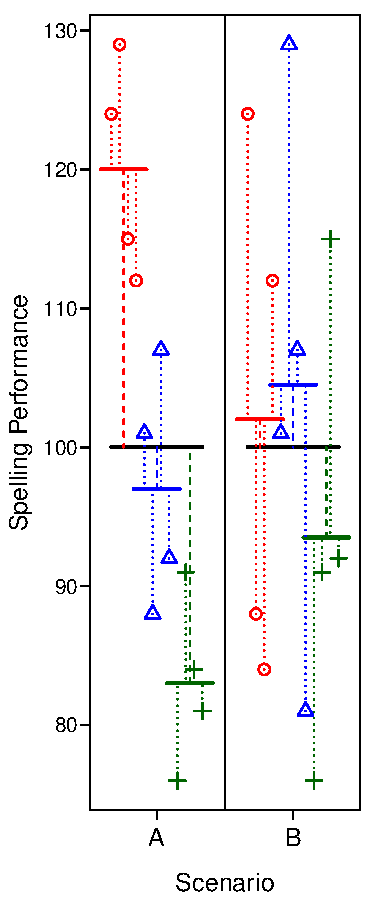
\includegraphics[scale=.5]{08_glm_img/spelling-05.pdf}
\end{column}

\begin{column}{.73\columnwidth}
\(Y_{ij} - \mu = A_i + S(A)_{ij}\)

\begin{block}{Scenario A}
\(SS_{A} = 2792\)

\(SS_{S(A)}=526\)

\(SS_{A} + SS_{S(A)}=3318\)
\end{block}

\begin{block}{Scenario B}
\(SS_{A} = 266\)

\(SS_{S(A)}=3052\)

\(SS_{A} + SS_{S(A)}=3318\)
\end{block}
\end{column}
\end{columns}
\end{frame}

\begin{frame}[label={sec:org99e0600}]{Mean Square and Degrees of Freedom}
\begin{columns}
\begin{column}{.27\columnwidth}
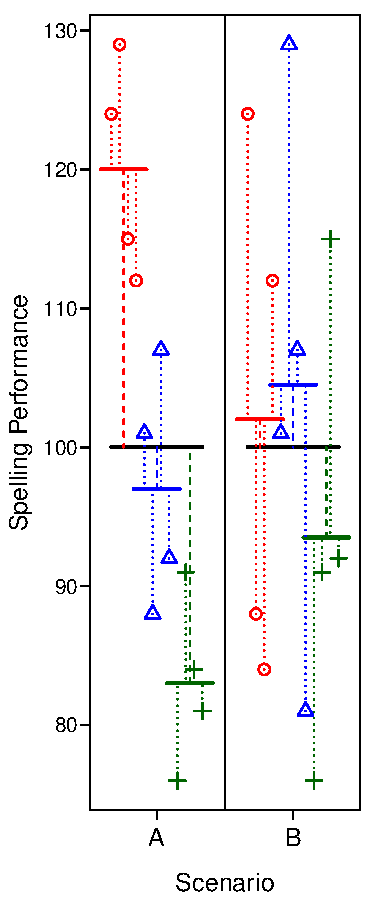
\includegraphics[scale=.5]{08_glm_img/spelling-05.pdf}
\end{column}

\begin{column}{.73\columnwidth}
\begin{block}{Degrees of Freedom (df)}
The number of observations that are ``free to vary''.

\(df_{A} = K-1\)

\(df_{S(A)} = N-K\)

where \(N\) is the number of subjects and \(K\) is the number of groups.
\end{block}

\begin{block}{Mean Square (MS)}
A sum of squares divided by its degrees of freedom.

\(MS_A = \frac{SS_A}{df_A} = \frac{2792}{2} = 1396\)

\(MS_{S(A)} = \frac{SS_{S(A)}}{df_{S(A)}} = \frac{526}{9} = 58.4\)
\end{block}
\end{column}
\end{columns}
\end{frame}

\begin{frame}[label={sec:orge81a0ef}]{The \(F\)-ratio}
\begin{columns}
\begin{column}{.4\columnwidth}
\begin{block}{F density function}
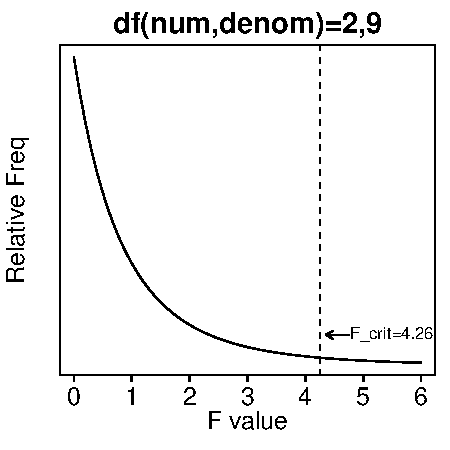
\includegraphics[width=.9\linewidth]{f-ratio.pdf}

If \(F_{obs} > F_{crit}\), then reject \(H_0\)
\end{block}
\end{column}

\begin{column}{.58\columnwidth}
\begin{block}{F ratio}
A ratio of mean squares, with df\_\{numerator\} and df\_\{denominator\} degrees of freedom.

\(F_A = \frac{MS_A}{MS_{S(A)}} = \frac{1396}{58.4} = 23.886\)
\end{block}

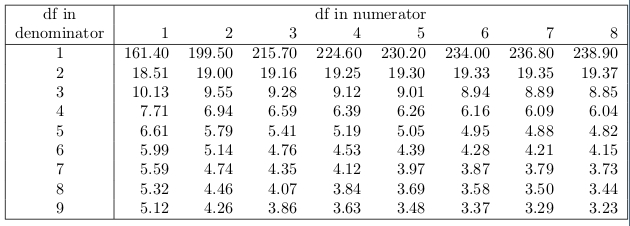
\includegraphics[width=.9\linewidth]{08_glm_img/ftable.jpg}
\end{column}
\end{columns}
\end{frame}

\begin{frame}[fragile,label={sec:org2c33abb}]{Density/Quantile functions for \emph{F}-distribution}
 \begin{small}

\begin{center}
\begin{tabular}{ll}
name & function\\
\hline
\texttt{pf(x, df1, df2, lower.tail = FALSE)} & density (get \(p\) given \(F_{obs}\))\\
\texttt{qf(p, df1, df2, lower.tail = FALSE)} & quantile (get \(F_{crit}\) given \(p\))\\
\hline
\end{tabular}
\end{center}

\end{small}
\end{frame}

\begin{frame}[label={sec:org4be8ac6}]{Summary Table}
\begin{columns}
\begin{column}{.27\columnwidth}
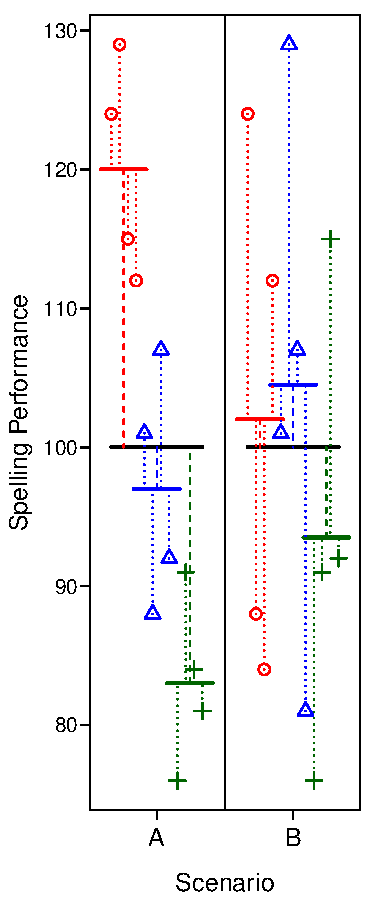
\includegraphics[scale=.5]{08_glm_img/spelling-05.pdf}
\end{column}

\begin{column}{.73\columnwidth}
\begin{block}{Scenario A}
\begin{scriptsize}
\begin{center}
\begin{tabular}{lrrrrrl}
\hline
Source & \(df\) & \(SS\) & \(MS\) & \(F\) & \(p\) & Error\\
\hline
\(\mu\) & 1 & 120000 & 120000.0 & 2053.232 & <.001 & \(S(A)\)\\
\(A\) & 2 & 2792 & 1396.0 & 23.886 & <.001 & \(S(A)\)\\
\(S(A)\) & 9 & 526 & 58.4 &  &  & \\
\hline
Total & 12 & 123318 &  &  &  & \\
\hline
\end{tabular}
\end{center}
\end{scriptsize}
\end{block}

\begin{block}{Scenario B}
\begin{scriptsize}
\begin{center}
\begin{tabular}{lrrrrrl}
\hline
Source & \(df\) & \(SS\) & \(MS\) & \(F\) & \(p\) & Error\\
\hline
\(\mu\) & 1 & 120000 & 120000.0 & 353.878 & <.001 & \(S(A)\)\\
\(A\) & 2 & 266 & 133.0 & .392 & .687 & \(S(A)\)\\
\(S(A)\) & 9 & 3052 & 339.1 &  &  & \\
\hline
Total & 12 & 123318 &  &  &  & \\
\hline
\end{tabular}
\end{center}
\end{scriptsize}
\end{block}
\end{column}
\end{columns}
\end{frame}


\begin{frame}[fragile,label={sec:orgb0a9f55}]{Overview of One-Way ANOVA}
 \begin{columns}
\begin{column}{.52\columnwidth}
\begin{scriptsize}
\begin{enumerate}
\item Write the GLM: \(Y_{ij} = \mu + A_i + S(A)_{ij}\)
\item Write down the estimating equations:
\begin{itemize}
\item \(\hat{\mu} = Y_{..}\)
\item \(\hat{A_i} = Y_{i.}-\hat{\mu}\)
\item \(\widehat{S(A)_{ij}} = Y_{ij}-\hat{\mu}-\hat{A_i}\)
\end{itemize}
\item Compute estimates for all terms in model.
\item Create \emph{decomposition matrix.}
\item Compute \(SS\), \(MS\), \(df\).
\begin{itemize}
\item \(df_{\mu}=1\)
\item \(df_{A}=K-1\)
\item \(df_{S(A)}=N-K\)
\item \(MS=SS/df\)
\end{itemize}
\item Construct a summary ANOVA table.
\item Compare F\_\{obs\} with F\_\{crit\}.
\end{enumerate}
\end{scriptsize}
\end{column}

\begin{column}{.45\columnwidth}
\begin{block}{R}
use the \texttt{aov()} function, e.g.:

\begin{minted}[frame=lines,fontsize=\scriptsize,linenos,tabsize=2]{r}
spelling$A <- factor(spelling$A)
mod <- aov(Y ~ A, data = spelling)
summary(mod)
\end{minted}

\begin{tiny}

\url{http://talklab.psy.gla.ac.uk/stats/onefactoranova.html#sec-3-2}

\end{tiny}
\end{block}
\end{column}
\end{columns}
\end{frame}


\begin{frame}[label={sec:org8c29850}]{Other GLMs}
\begin{itemize}
\item one-sample \(t\)-test
\(Y_i - c = \beta_0 + e_i\)

\item two-sample \(t\)-test
\(Y_i = \beta_0 + \beta_1 X_i + e_i\)
\begin{itemize}
\item where \(X_i \in \left(0, 1\right)\)
\end{itemize}

\item paired-samples t-test
\(Y_{1i} - Y_{2i} = \mu + e_i\)

\item simple linear regression
\(Y_{i} = \beta_0 + \beta_1 X_i + e_i\)

\item multiple regression
\(Y_{i} = \beta_0 + \beta_1 X_{1i} + \beta_2 X_{2i} + e_i\)

\item ANCOVA
\(Y_{i} = \beta_0 + \beta_1 X_{1i} + \beta_2 X_{2i} + \beta_3 X_{1i} X_{2i} + e_i\)
\begin{itemize}
\item where \(X_{1i} \in \left(0, 1\right)\) and \(X_{2i} \in \mathbb{R}\)
\end{itemize}
\end{itemize}
\end{frame}
\end{document}
